\section{Model Analysis}
\subsection{Strengths and Weaknesses}

\textit{\textbf{Strengths.}}
% \subsection{Strengths}
\begin{enumerate}
    \item \textbf{Close to real-world scenarios: }In problem 1, we utilized the three gate mechanisms and Cell state of LSTM to simulate the human processes of memory formation and forgetting, closely approximating real-life scenarios.

    \item \textbf{Temporal memory capability: }The LSTM model captures and remembers long-term dependencies through its Cell state, enabling it to effectively process long sequences of data and form a memory of the data throughout the competition process.
    \item \textbf{Momentum-based model representation: }In problem 2, we modeled the LSTM as a mathematical model based on momentum, providing a more formal analysis of the intrinsic relationship between the LSTM model and the momentum model.

    \item \textbf{Strong generalization capability: }We performed dimensionality reduction on the data from the competition, extracting some mutually independent factors to be used as inputs for the model, thereby enhancing its generalization capabilities when faced with new data.
    \item \textbf{Objective results: }The results of the model are quantifiable and can be described by mathematical representations so that speculative thinking is not required.
\end{enumerate}

% \subsection{Weaknesses}
\textit{\textbf{Weaknesses.}}
\begin{enumerate}
    \item \textbf{The momentum modeling is not comprehensive: }Due to the influence of many non-intuitive factors in the competition process, even though our LSTM model considers many factors in the game, it still cannot accurately model the momentum of players throughout the competition.
    \item \textbf{Insufficient prediction accuracy: }To further improve accuracy, we need to use more game data to enable our deep learning model LSTM to learn more information about the games.

\end{enumerate}


\subsection{Sensitivity Analysis}
To validate the model’s sensitivity, we simulated scenarios of missing data by selectively removing portions of the input data. Specifically, we sequentially excluded several variables that were identified to have the largest gradient contributions in Section \ref{sec:factor_contribution}. The model’s accuracy decreased by only 2\% when the variable with the greatest gradient contribution was removed. When five variables were excluded, the model still maintained an accuracy of 84\%. These results indicate that our model can adapt to partial data missingness, demonstrating strong robustness and resilience. The related experimental analysis results are presented in Figure \ref{fig:sensitivity_analysis}.

%%%%%%%%%
%%% 小标文字
%%%%%%%%%

\begin{figure}[htbp]
  \centering
  \subfigure[The accuracy of LSTM changing with the number of factors]
  {%
    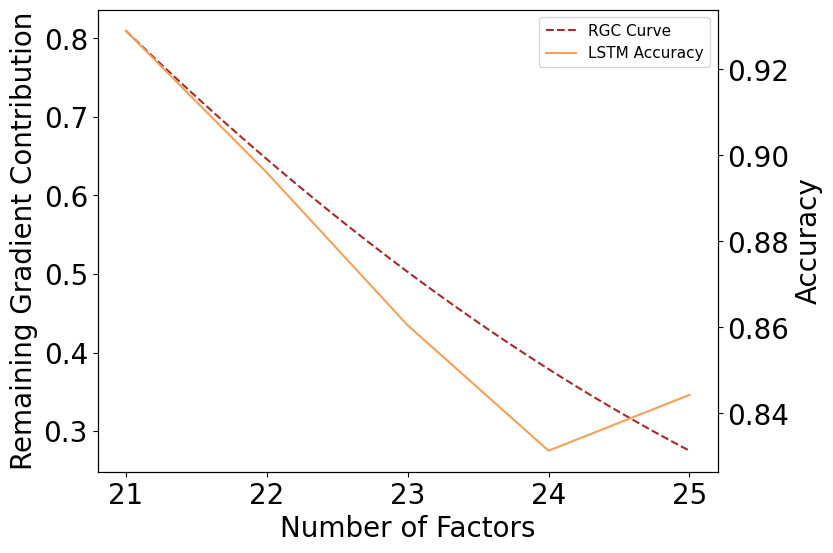
\includegraphics[width=0.45\textwidth]{figure/output2.png}
    \label{fig:lstm_acc_sensitivity_analysis}
  }
  % \hfill
  \hspace{1cm}
  \subfigure[The loss of LSTM changing with the number of factors]{%
    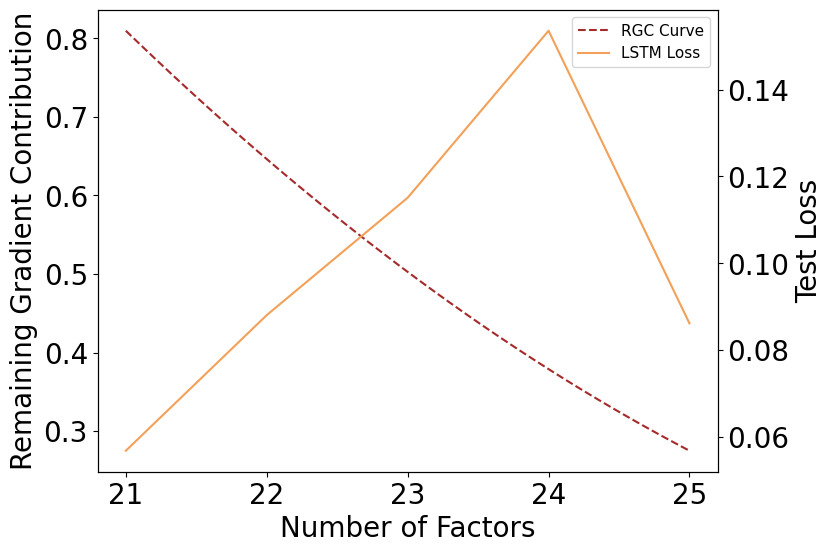
\includegraphics[width=0.45\textwidth]{figure/output1.png}
    \label{fig:lstm_loss_sensitivity_analysis}
  }
  \caption{Figures for Sensitivity Analysis}
  \label{fig:sensitivity_analysis}
\end{figure}